\section{Results}

\subsection{Data usage across operating systems and scenarios}

Total network data usage across all operating systems and applicable scenarios for performed tasks, is presented on charts in Figures~\ref{fig-setup-chart}--\ref{fig-apps-chart}. To keep the results comparable and avoid dominance by bulk transfers, we excluded traffic to domains used for app and system update payload delivery (large binary downloads), though this exclusion was not perfect and some residual update-related traffic remains in the dataset. Generally, we expect lower network traffic in configurations with fewer Google services present.

\begin{figure}
	\includegraphics[width=\textwidth]{images/setup-data-usage.eps}
	\caption{Task 0: Initial setup data usage} \label{fig-setup-chart}
\end{figure}

Figure \ref{fig-setup-chart} illustrates network activity during initial device setup. As expected, stock Android shows the highest data usage. The modest reductions between privacy-adjusted scenarios indicate that configuration choices provide little control over automatic updates and background synchronization. Across all distributions, variations align with service architecture: configurations incorporating more Google services generate proportionally higher traffic, while de-Googled baselines demonstrate substantially reduced exchange. LineageOS with official Google Play Services generates substantially less traffic than stock Android due to its more minimal base system, yet remains considerably higher than configurations without proprietary Google services, with the microG variant and Google-free installation achieving notable further reductions. On GrapheneOS, Scenario B demonstrates that even when sandboxed Google Play Services are installed and granted network and background permissions, they remain largely inactive when not deliberately invoked, contrasting with the persistent background activity characteristic of integrated GMS deployments.

\begin{figure}
	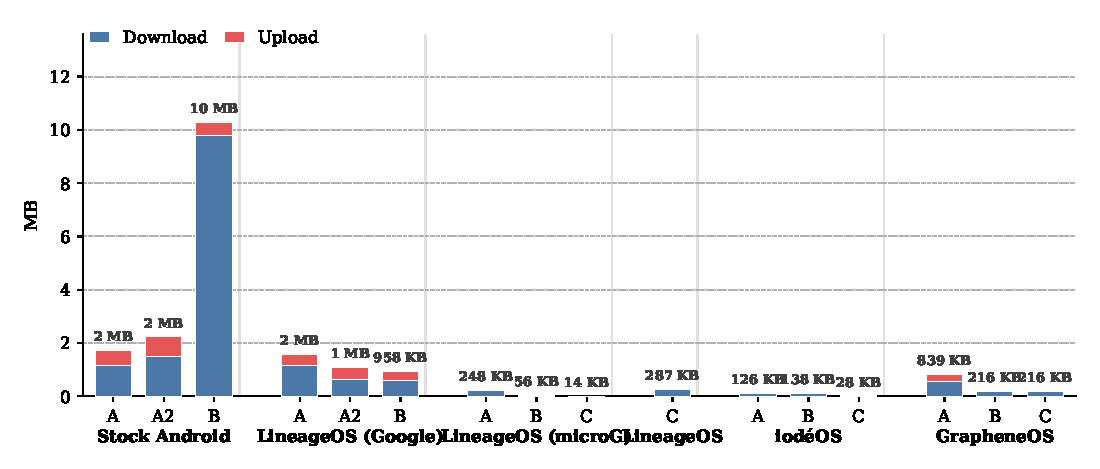
\includegraphics[width=\textwidth]{images/idle-data-usage.eps}
	\caption{Task 1: Idle data usage} \label{fig-idle-chart}
\end{figure}

Network activity observed during system idle following a reboot is presented in Figure \ref{fig-idle-chart}. Stock Android again shows the highest data usage, though Scenario B exhibits unexpectedly elevated traffic compared to both Scenario A2 and Scenario A. This anomaly stems from substantial background communication with www.gstatic.com, likely triggered by automatic updates or application background activity during the measurement time.

LineageOS in Scenario C similarly deviate from anticipated patterns, generating more idle traffic than its microG variant. LineageOS made connections to agnss.goog (Google Assisted GNSS) and www.gstatic.com. The agnss.goog endpoint was also observed in LineageOS (microG) during other measurement tasks, indicating that the entire LineageOS family retains this Google-dependent location mechanism. Other alternative distributions either replace this component with independent implementations or allow users to disable it entirely. GrapheneOS exhibits virtually identical idle traffic in Scenarios B and C, confirming that sandboxed Google Play Services remain dormant when not actively invoked.

\begin{figure}
	\includegraphics[width=\textwidth]{images/apps-data-usage.eps}
	\caption{Task 2: Basic apps interactions data usage} \label{fig-apps-chart}
\end{figure}

Figure~\ref{fig-apps-chart} shows network activity during basic app interactions that should not require Internet connectivity. Stock Android dominates with substantial data usage mostly by uncontrolled updates. All alternative distributions demonstrate dramatically lower traffic, with de-Googled configurations remaining effectively silent. Notably, whenever official Google Play Services were present and a Google account logged in at least a single request to Google infrastructure occurred.

\subsection{Domain distribution and Google dependencies}

\begin{figure}
	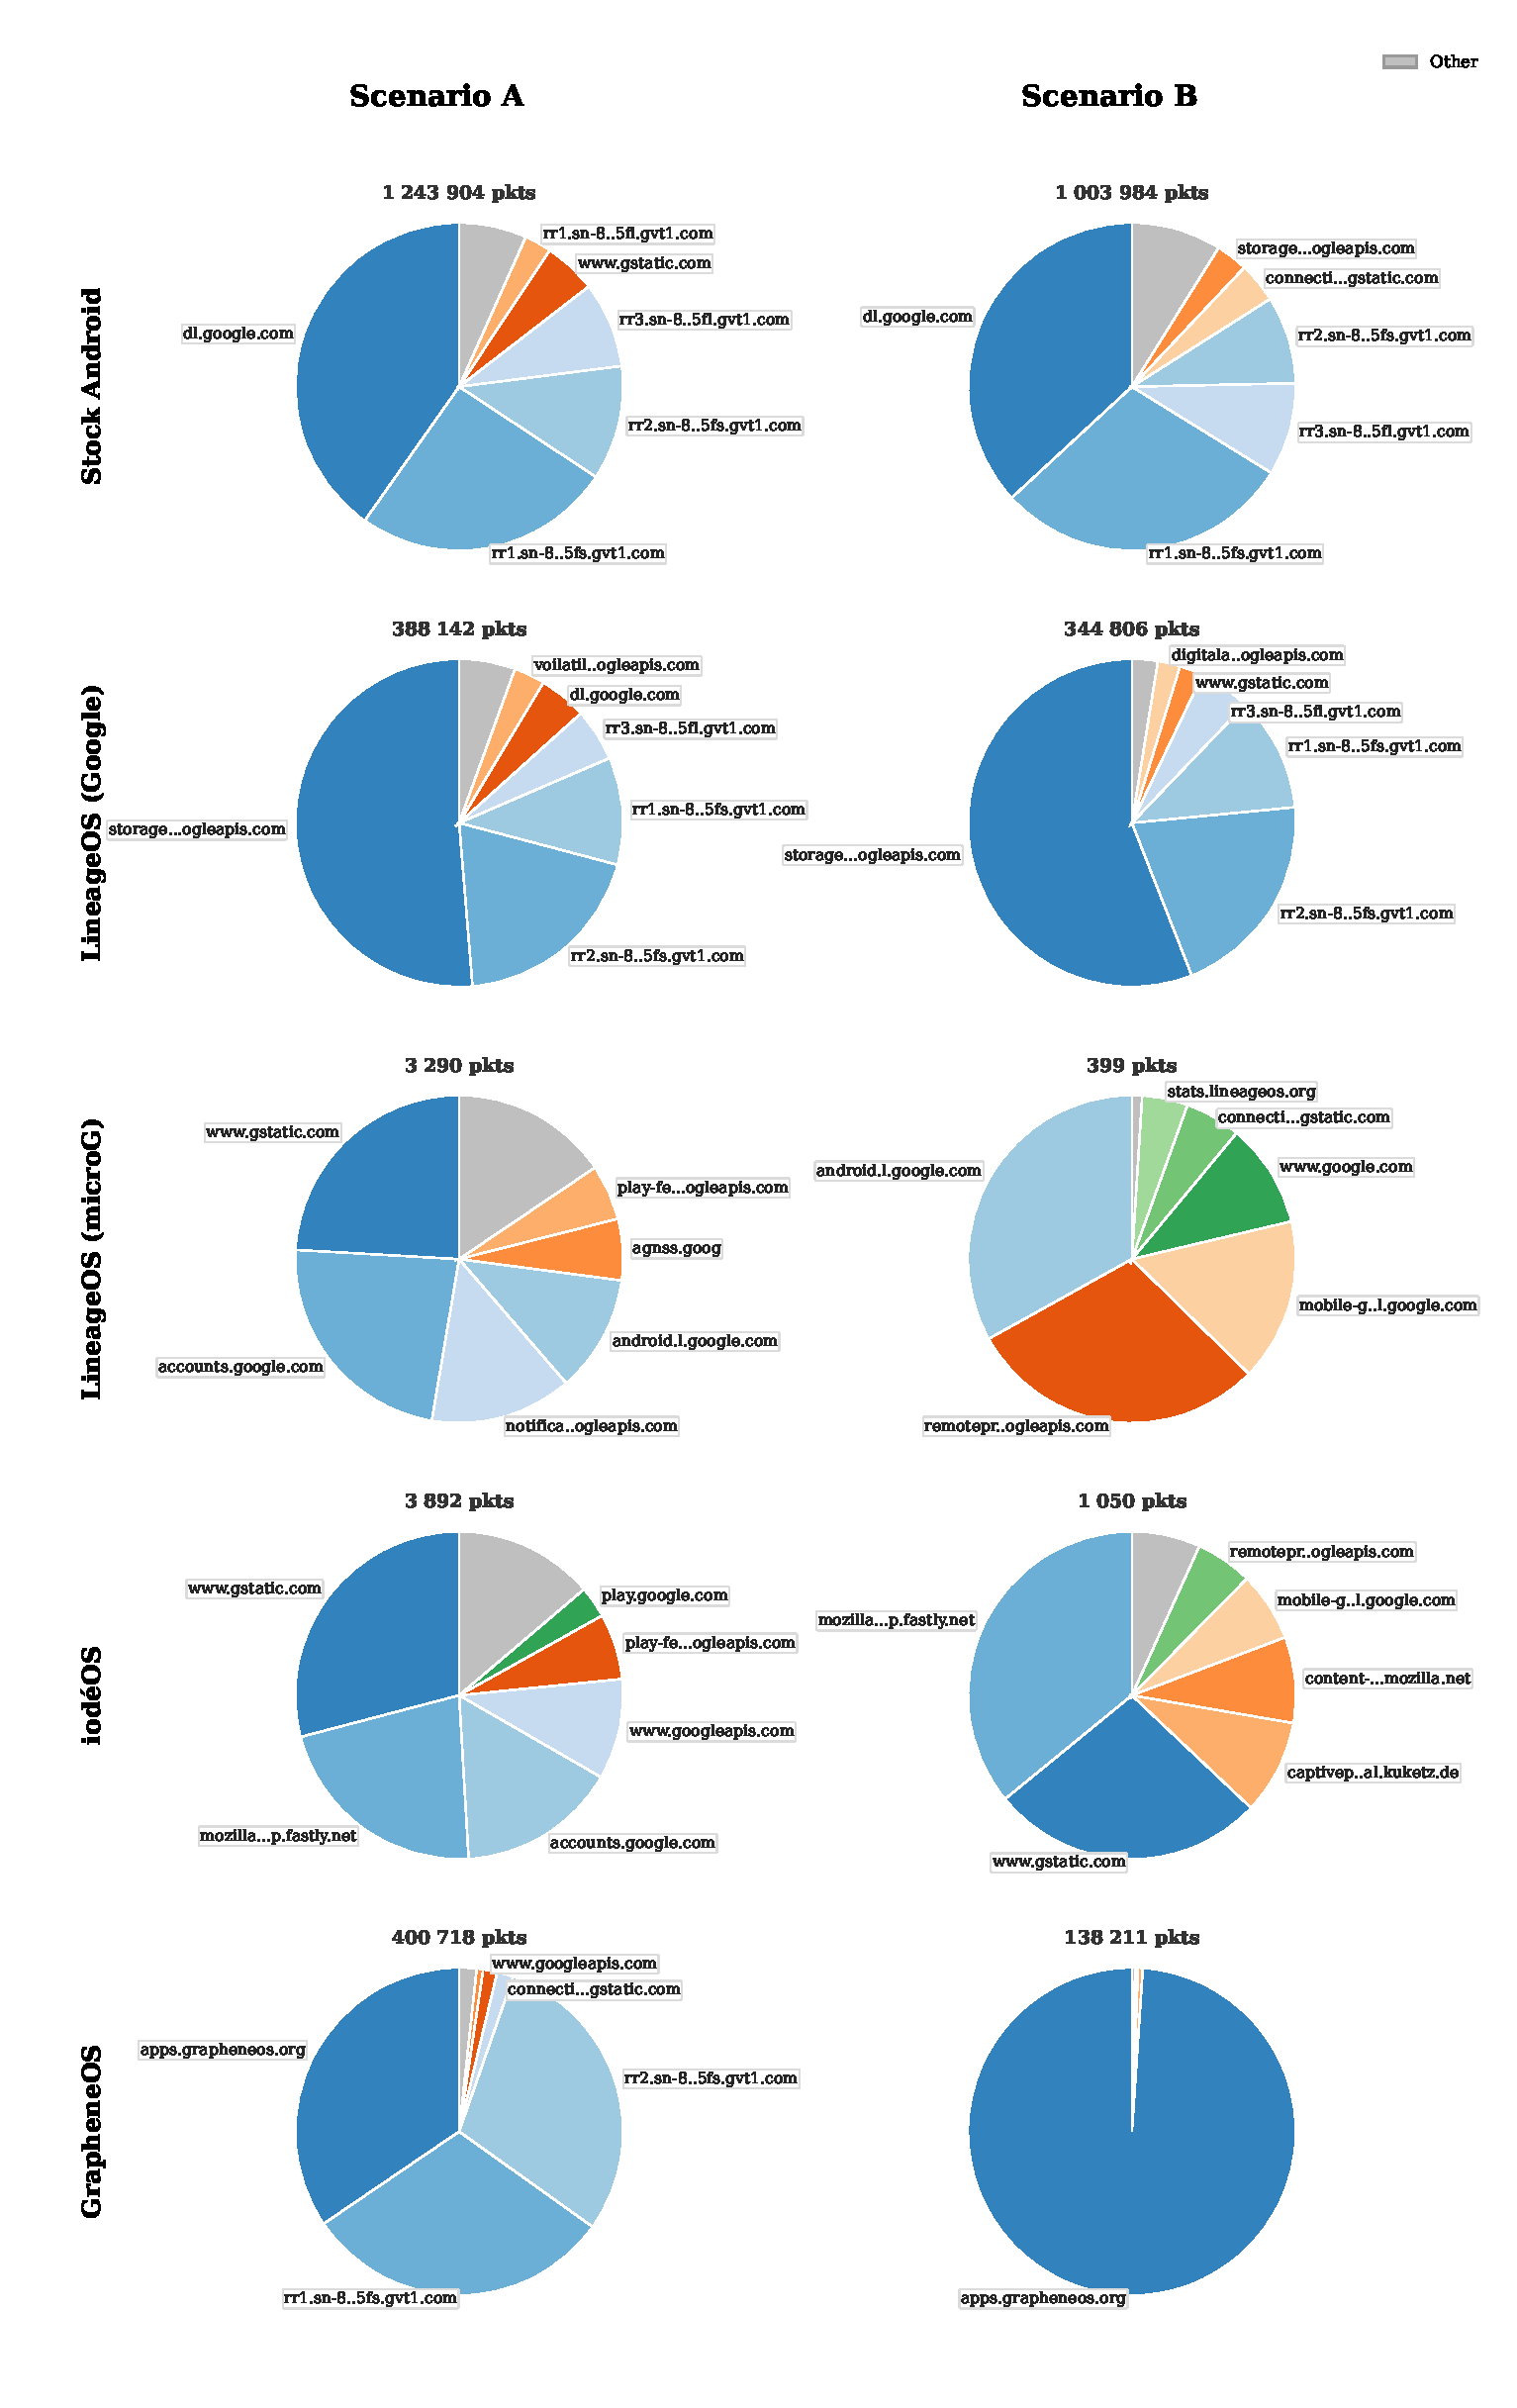
\includegraphics[width=\textwidth]{images/domains.eps}
	\caption{Domain-level distribution of network packets for scenarios A (with Google account) and B (without Google account, but Google Services present), aggregated over all tasks. Each pie shows the top domains by packet count for a given operating system and scenario.} \label{fig-domains-chart}
\end{figure}

Figure \ref{fig-domains-chart} presents the domain-level distribution of network traffic for Scenarios A and B. They were selected as the most realistic configurations incorporating essential Google functionality while differing in account linkage and privacy-related settings. Overall traffic is dominated by large content transfers, as systems download necessary resources and updates. Stock Android contacts the widest range of Google domains, spreading traffic across many different endpoints. Alternative systems show less Google communication, though patterns vary by design. GrapheneOS makes more requests than microG-based systems because it downloads Google services on demand from its own app store rather than having them preinstalled. IodéOS and LineageOS with microG reach fewer Google servers overall, as microG minimizes Google connectivity while still enabling basic features. IodéOS additionally relies on some Mozilla infrastructure not present in other systems.

Table~\ref{tab:domains-mechanisms} shows the infrastructure dependencies for basic system functions. LineageOS variants remain closest to stock Android, relying entirely on Google servers for connectivity checks, remote provisioning, and location assistance. IodéOS adopts an intermediate position, using independent infrastructure for connectivity checks while still depending on Google for remote provisioning and location services. GrapheneOS demonstrates the strongest de-Googling, substituting all three functions with its own or independently operated infrastructure. Both iodéOS and GrapheneOS expose these mechanisms through explicit system settings toggles, though GrapheneOS offers more granular control: users may choose between its independent proxy infrastructure and official Google servers for each function, with defaults configured to avoid Google connections entirely.

\begin{table}
	\caption{Domains observed for connectivity check, remote provisioning, and location assistance.}\label{tab:domains-mechanisms}
	\centering
	\resizebox{\linewidth}{!}{%
		\begin{tabular}{|l|l|l|l|}
			\hline
			System & Connectivity check & Remote provisioning & Location assistance\\
			\hline
			Stock Android & connectivitycheck.gstatic.com & -- & supl.google.com agnss.goog\\
			LineageOS & connectivitycheck.gstatic.com & remoteprovisioning.googleapis.com & supl.google.com agnss.goog\\
			iodeOS & captiveportal.kuketz.de & remoteprovisioning.googleapis.com & supl.google.com\\
			GrapheneOS & connectivitycheck.grapheneos.network & remoteprovisioning.grapheneos.org & gs-loc.apple.grapheneos.org\\
			\hline
		\end{tabular}%
	}
\end{table}

\subsection{Additional findings}

Beyond aggregate traffic measurements, we examined specific data transmissions revealed through TLS interception and payload analysis. Some observations were gathered earlier on Android 14 and could not be reconfirmed on Android 16, as the Frida-based method we employed became unsuccessful, though we expect the general patterns to persist. GrapheneOS blocked all our instrumentation attempts, so we cannot verify what data these requests contained. However, the substantially lower request volume suggests sandboxed Google Play Services likely transmit less complete or authentic information.

\paragraph{Device identifiers.}
Android's checkin mechanism transmits device identifiers to Google infrastructure. On stock systems, this includes the real IMEI and hardware serial number. In contrast, microG employs a privacy-preserving approach by generating randomized, rotating identifiers including fake IMEIs (consistently prefixed with \texttt{35503104}), MAC addresses (with OUI \texttt{b4:07:f9}), and a synthetic serial key displayed in microG settings. The Android ID field in microG requests is frequently empty or zeroed. However, microG still transmits authentic device characteristics including model, Android version, and timezone, enabling functional compatibility while obscuring persistent hardware identifiers.

\paragraph{Application telemetry.}
We observed requests to \texttt{app-measurement.com} on systems with Google services present, most on stock Android. These transmissions contained application package names, installation sources (Google Play, Aurora Store, manual), app versions and system theme preference. Information about installed applications was transmitted even for apps that were never launched.

\paragraph{Advertising ID.}
The Google Advertising ID (ADID) was observed in multiple requests on stock Android, formatted as a UUID. This value remained constant across different requests, confirming its persistence as a cross-app tracking mechanism. After manual reset in system settings, the ADID was transmitted as zeros, indicating the identifier was actually cleared rather than regenerated immediately.

\paragraph{Network-based geolocation in microG.}
When enabled by the user, microG performs network geolocation without Google infrastructure by querying a selected provider, in our case \texttt{api.positon.xyz}. The request transmits nearby cell tower data and returns approximate coordinates. Location fixes were obtained almost immediately after enabling this feature, compared to substantially slower determination prior to activation.

\paragraph{App store comparison.}
We compared Google Play Store with Aurora Store, a popular application source in alternative Android distributions, by downloading the same application from both stores. Both retrieved identical packages from the same Google CDN infrastructure. However, the Play Store generated 106 requests while Aurora Store produced 93 requests, omitting Google telemetry connections, but adding lookups to Exodus Privacy and Plexus databases for tracker analysis and compatibility ratings. Aurora achieves functional equivalence by mimicking Play Store user agents and headers, though with shared anonymous credentials rather than personal account.

\subsection{Google Takeout}

Following testing scenarios where we logged into a Google account, we submitted Google Takeout requests and analyzed the Android device data. Our selection covered three distinct Google service configurations: Stock Android and LineageOS with GMS as systems incorporating official Google services, LineageOS with microG as an open source reimplementation (IodéOS includes an identical microG version), and GrapheneOS as a representative of sandboxed Google Play. For every logged in system, an entry appeared in \texttt{devices.json} containing device model, OS version, country, language, registration timestamp, and last activity time. However, the depth of telemetry varied considerably across configurations.

Both systems using official Google services reported a large list of installed apps. GrapheneOS reported only four preinstalled applications, two of which were GrapheneOS specific. In contrast, microG did not create any app-related entry in Takeout. Additionally, Stock Android and LineageOS with GMS both transmitted authentic hardware identifiers including IMEI and serial number. GrapheneOS submitted a falsified serial number and omitted IMEI entirely. Again, microG did not create additional device-related entry, so these identifiers were not present.

A Pixel specific telemetry directory, present only for Stock Android and LineageOS with GApps, contained extensive hardware monitoring data including power measurements, Wi-Fi signal logs, battery capacity readings, thermal samples, and battery cycle entries. LineageOS reported less granular telemetry than Stock Android, indicating that while basic Pixel telemetry infrastructure remains functional, the depth of hardware monitoring is reduced compared to the proprietary stock implementation.